\subsection{Multipoles (\textbf{L3})}

\subsubsection{\hyperref[Spherical Multiple Moment]{Spherical Multiple Moment}}

Consider the system where you have point charges $+q$ at $(a, 0,0)$ and $(0, a, 0)$ and charges $-q$ at $(-a, 0,0)$ and $(0,-a, 0)$. Derive the spherical multiple moment $q_{l, m}$ and write down the first two non vanishing terms. Express the charge density in spherical coordinates and check that the integral over these densities produce the appropriate total charge.

\subsubsection{\hyperref[Multiple Moments in Cartesian Coordinates]{Multiple Moments in Cartesian Coordinates}}

\begin{enumerate}
	\item Prove that $Q_{i j}$ is traceless.
	\item Assume that $q, \vec{p}, Q_{i j}$ are in a specific coordinate system. Now find the new quantities in a coordinate system which is related to the previous one by an $\vec{R}$ displacement.
	Assume now that you have charges $q$ at $(0, a, 0)$ and $(0,0, a)$ and charge $-q$ at $(a, 0,0)$
	\item Find $q, \vec{p}, Q_{i j}$ and check that the later one is traceless.
	\item Can you find a coordinate system such that $\vec{p}^{\prime}=0 ?$ If yes what is the displacement vector $\vec{R} ?$
\end{enumerate}

\subsubsection{\hyperref[Exterior Multipoles for a Specified Potential on a Sphere]{Exterior Multipoles for a Specified Potential on a Sphere}} 

Let $\Phi (R, \theta,\phi)$ be specified values of the electrostatic potential on the surface of a sphere. Show that the general form of an exterior, spherical multipole expansion implies that,

\begin{equation}
	\Phi[\vec{r}] = \sum_{l=0}^{\infty} \sum_{m=-l}^{l} \left(\frac{R}{r}\right)^{l+1} Y_{l,m} [\Omega]\int d \Omega ' \Phi [R, \Omega '] Y^{*}_{l',m'}[\Omega ']
\end{equation}

For $r > R$. Given the previous potential expression, imagine the eight octants of a spherical shell which are maintained at alternating electrostatic potentials  $\pm V$ as shown below in the following picture:

\begin{figure}[htbp!]
	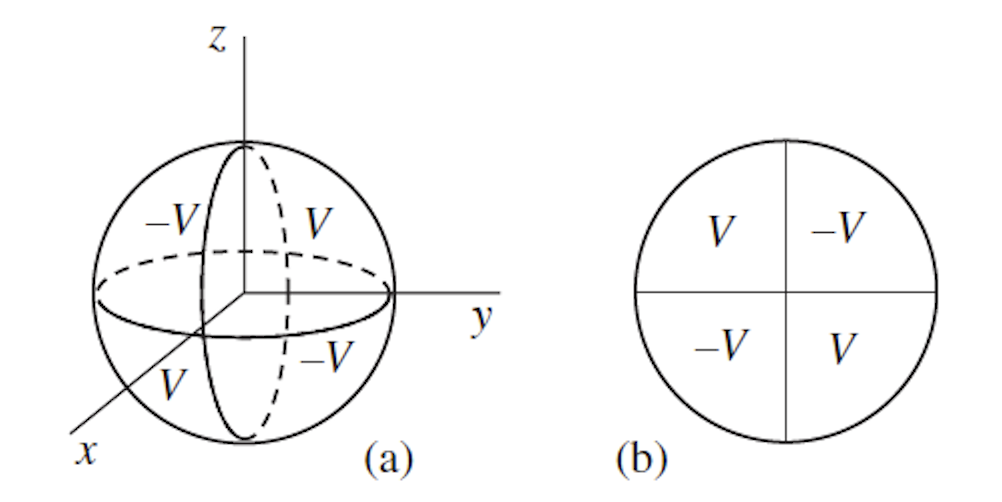
\includegraphics[width=8cm]{figures/shells.png}
	\centering
	\caption{Potential distribution across the octants.}
\end{figure}

Where view $a$ is in perspective and $b$ is looking down the $z$ axis from above. Use the results from previous section to find the asymptotic ($r \rightarrow \infty$) form of the potential produced by this shell configuration.

\subsubsection{\hyperref[Radiating Fidget Spinner]{Radiating Fidget Spinner}}

Three identical point charges $q$ are at the corners of an imaginary equilateral triangle that lies in the $x-y$ plane. The charges rotate with constant angular velocity $\omega$ around the $z$ -axis, which passes through the center of the triangle. Find the angular distribution of electric dipole, magnetic dipole, and electric quadrupole radiation (treated separately) produced by this source.

